%%%% paper/draft_v1.tex -- DRAFT v1 (2026-11-04), IJCAI-27 template (ijcai27.sty, named.bst)
%%%%
%%%% Number policy: every number below is copied from a file in this repo. Each key number has
%%%% a "% SRC:" comment naming the file and, where one exists, the result commit. Cells whose raw
%%%% trajectories are lost (amend22/24/26) are reported under the metric they were registered with
%%%% (inside the goal at the final instant T) and are marked "to be regenerated under the settled
%%%% metric". Anything not computed is written as future work. See paper/review_draft.md.
%%%%
%%%% Two experimental configurations are used and must never be mixed in one comparison:
%%%%   Config G ("crossover geometry", amend21/22): one arena for N=25..200, d_safe 0.70 (0.55 for
%%%%            real as a second margin), 10 seeds, A100, inside-at-T metric; raw logs LOST.
%%%%   Config S ("stage-1 config", amend11/33/34/38): N=100, d_safe 0.55, 5 seeds, CPU; raw logs
%%%%            kept, settled metric computed exactly.

\typeout{draft_v1 -- staleness-limited safety in MFG+CBF swarms}

\documentclass{article}
\pdfpagewidth=8.5in
\pdfpageheight=11in
\usepackage{ijcai27}

\usepackage{times}
\usepackage{soul}
\usepackage{url}
\usepackage[hidelinks]{hyperref}
\usepackage[utf8]{inputenc}
\usepackage[small]{caption}
\usepackage{graphicx}
\usepackage{amsmath}
\usepackage{amsthm}
\usepackage{booktabs}
\usepackage{multirow}
\usepackage{algorithm}
\usepackage{algorithmic}
\usepackage[switch]{lineno}
\linenumbers
\urlstyle{same}

\graphicspath{{../results/overnight_figures/}}

\newcommand{\Tf}{T_{\mathrm{frame}}}
\newcommand{\tslot}{t_{\mathrm{slot}}}
\newcommand{\dsafe}{d_{\mathrm{safe}}}
\newcommand{\ci}[2]{\,[#1,\,#2]}

\pdfinfo{
/TemplateVersion (IJCAI.2027.0)
}

\title{Staleness, Not Crowding: Where Delay Compensation Belongs\\in a Decentralized Mean-Field-Game Swarm with a Barrier Safety Filter}

\author{
    Anonymous Submission
    \affiliations
    \emails
}

\begin{document}

\maketitle

\begin{abstract}
We study a decentralized drone swarm that routes with an offline-solved mean-field-game (MFG)
controller and enforces separation with a per-agent control-barrier-function (CBF) safety filter.
Agents see their neighbours only through UWB range and vision bearing, broadcast over a TDMA
channel whose frame length grows linearly with the swarm size $N$. In controlled simulations
with drone-sized keep-out distances, we show three things.
(1) Collisions are caused by the staleness of neighbour estimates, not by density: with
the delay removed but sensor noise kept, no agent ever comes within 0.30\,m of another up to
$N{=}200$. At a fixed $N{=}100$, lengthening only the TDMA slot reproduces the collision rate of
the $N$-sweep at equal frame length.
(2) Delay compensation has to be fed to the CBF layer, not the MFG layer. Feeding even an oracle
estimate to the MFG density term changes safe success by exactly $0.000$, while feeding it to the
CBF recovers the whole gap. The MFG layer earns its place through liveness: $+0.32$ settled
success over a CBF-only swarm with zero collisions.
(3) A learned, conformally calibrated uncertainty margin (``$\sigma$-CBF'') does not beat a
constant margin. It wins slightly at $N{=}150$ ($+0.039$), loses at $N{=}200$ ($-0.189$), and
its calibration coverage drops from 0.95 offline to 0.77 in closed loop.
A pooled-$N$ learned predictor recovers 88\% of the delay-induced safe-success gap at $N{=}100$
in the crossover geometry, and 14\% at $N{=}200$.
\end{abstract}

%=====================================================================
\section{Introduction}
%=====================================================================

Mean-field-game (MFG) controllers are a natural fit for large swarms. Each agent responds to a
density field rather than to every neighbour, and the equilibrium trades progress to a goal
against congestion~\cite{lasry2007mean,huang2006large,elamvazhuthi2019mean}. Deployed swarms,
however, add physics that the continuum model leaves out. Drones have a body size. Neighbours are
measured, not known: UWB ranging and camera bearing are noisy. Neighbour states arrive over a shared
radio. With time-division multiple access (TDMA), each agent broadcasts once per frame, and the
frame grows as $\Tf = N\,\tslot$. A larger swarm therefore acts on older information about its
neighbours.

A safety filter based on control barrier functions (CBFs)~\cite{ames2017cbf,wang2017safety} is
the standard way to add hard separation constraints to such a controller. It is only as good as
the neighbour positions it is given. This paper asks a narrow question, motivated by the design of
a two-layer MFG+CBF swarm: \emph{when realistic sensing and TDMA delay are added, what limits
safety, and where should delay compensation enter the stack?}

\paragraph{Contributions.}
We show, in controlled simulation, that the staleness of TDMA communication, not crowding, limits
the safety of a decentralized MFG+CBF swarm. Delay compensation must be given to the CBF layer,
not the MFG layer. A learned margin with a conformal guarantee does not fix the problem.
Concretely:
\begin{enumerate}
\item \textbf{A controlled characterization of staleness-limited safety with an isolated mechanism.}
  Removing only the delay removes every collision up to $N{=}200$ (Sec.~\ref{sec:mech}). A
  pure-staleness sweep at fixed $N$ matches the collision rate of the $N$-sweep at equal
  $\Tf$, while the completeness loss at large $N$ tracks density (Sec.~\ref{sec:barrier}).
\item \textbf{A separation of layer roles under delay.} Compensation fed to the MFG density
  term changes safety by exactly zero, even with an oracle. Fed to the CBF, it recovers the whole
  gap. The MFG layer pays for itself in liveness, not safety: it prevents the deadlocks that a
  CBF-only swarm falls into (Sec.~\ref{sec:layers}).
\item \textbf{A negative result on uncertainty-as-guarantor.} A per-neighbour error model ranks
  risky neighbours well but does not size their errors. The conformal margin built on it loses
  coverage in closed loop, and the resulting $\sigma$-CBF does not beat a constant margin at the
  density it was built for (Sec.~\ref{sec:sigma}).
\end{enumerate}
We also report what the swarm does \emph{not} achieve. Even with no delay, about 8\% of agents
(exact positions) and 20\% (with sensor noise) settle on the rim of the goal disc rather than
inside it (Sec.~\ref{sec:metric}). The settled metric and a goal-tolerance band are therefore part
of the evaluation protocol, not an afterthought.

%=====================================================================
\section{Related Work}
%=====================================================================

\paragraph{Mean-field games for swarms.}
MFGs couple a Hamilton--Jacobi--Bellman equation for the value of a representative agent with a
Fokker--Planck equation for the population
density~\cite{lasry2007mean,huang2006large}, and they are solved numerically by finite
differences~\cite{achdou2010mean}. Mean-field models are widely used to design and analyse
swarm behaviour~\cite{elamvazhuthi2019mean}. These works assume that the density an agent responds
to is either the equilibrium density or a current local estimate. We keep the standard offline
MFG and ask what happens when each agent's \emph{local} density estimate is built from stale,
noisy neighbour broadcasts.

\paragraph{Control barrier functions for multi-agent safety.}
CBF-based quadratic programs enforce forward invariance of a safe set~\cite{ames2017cbf,ames2019cbf}
and scale to multi-robot collision avoidance through decentralized pairwise
constraints~\cite{borrmann2015control,wang2017safety}. We use such a filter unchanged as the
named safety layer.

\paragraph{Measurement-robust and delay-aware CBFs.}
Robust CBFs tighten the constraint by a bound on the model or measurement
error~\cite{jankovic2018robust}. Measurement-robust CBFs do the same for learned perception
errors~\cite{dean2020guaranteeing,cosner2021measurement}. Sampled-data and input-delay
formulations handle delay in the agent's own actuation
loop~\cite{singletary2020sampled,molnar2023delay}. In our setting the delay sits in the
\emph{neighbour} information, its size is set by the communication schedule ($\Tf = N\tslot$), and
it differs between neighbours (each has its own slot phase). A worst-case bound on it is
very conservative. We find that a constant margin larger than the best one makes an
\emph{uncompensated} swarm worse (Sec.~\ref{sec:method}).

\paragraph{Stochastic and conformal safety.}
Stochastic CBFs give probabilistic invariance under process noise~\cite{clark2021stochastic}.
Conformal prediction~\cite{vovk2005algorithmic,angelopoulos2021gentle} turns a learned
predictor into distribution-free prediction regions. It has been used to plan safely around
predicted agents~\cite{lindemann2023safe,dixit2023adaptive}. Our negative result
(Sec.~\ref{sec:sigma}) is a concrete instance of the known caveat: the coverage guarantee is
marginal and assumes exchangeability between calibration and deployment. A controller that
consumes the margin changes the distribution it is applied to.

\paragraph{How we differ.}
Prior work that feeds a neighbour predictor into a safety filter treats the predictor as an input
to one layer. Our question is \emph{which layer of a hierarchical controller} the compensation
belongs to. We answer it with a layer-split ablation under both a learned and an oracle estimate,
and the answer is a negative one for the MFG layer. Classical compensators (constant-velocity
extrapolation and a Smith-type model predictor~\cite{smith1957closer}) are included as comparators.

%=====================================================================
\section{System Model}
\label{sec:model}
%=====================================================================

\paragraph{Agents and task.}
$N$ point-mass agents with single-integrator dynamics, executed at $\Delta t = 0.01$\,s, cross a
wall through a single gate and must reach a goal disc.
% SRC: experiments/amend21_cells/*.yaml (dt_exec: 0.01); env/rollout.py ("single-integrator step")
Two agents collide when their true distance falls below $D_{\mathrm{COLL}} = 0.30$\,m, which
models the body of a 5-inch drone.
% SRC: prereg/prereg_projectA.md Sec.3 (D_COLLISION=0.30 m); CLAUDE.md (5" drones)
Speeds are clipped at $V_{\max} = 8$\,m/s.
% SRC: prereg/prereg_projectA.md Sec.3 (V_MAX=8.0)

\paragraph{Two-layer controller.}
\emph{Macro (MFG routing):} an offline MFG equilibrium is solved once per scenario and $N$ (Cesàro
mean over fictitious-play iterates). It gives a routing field $\Phi$ and an equilibrium density
$m^\star$. The nominal control of agent $i$ is
\begin{equation}
u_i^{\mathrm{nom}} = -\nabla\Phi(x_i) - c_{\mathrm{dens}}\nabla\big(\hat m_i - m^\star(x_i,t)\big)^2 + F_{\mathrm{bar}}(x_i;\hat x_{i\cdot}),
\end{equation}
where $\hat m_i$ is a kernel density estimate (bandwidth 0.60\,m, sensing radius 5\,m) built from
agent $i$'s \emph{estimates} $\hat x_{ij}$ of its neighbours, and $F_{\mathrm{bar}}$ is a bounded
soft barrier.
% SRC: control/law.py docstring; prereg/prereg_projectA.md Sec.2-3 (H_BANDWIDTH=0.60, R_SENSE=5.0)
\emph{Micro (CBF safety filter):} each agent solves a decentralized CBF-QP that keeps the nominal
control as close as possible while enforcing $\|\hat x_{ij} - x_i\| \ge \dsafe$ for every sensed
neighbour. Slack is minimized but allowed, so an infeasible QP never freezes an agent.
$\dsafe = D_{\mathrm{COLL}} + $ margin is the only safety knob.
% SRC: prereg/prereg_projectA.md Sec.2; control/cbf.py
Both layers consume the same neighbour estimates $\hat x_{ij}$, unless a layer-split ablation
gives each layer its own source (Sec.~\ref{sec:layers}).

\paragraph{Perception and TDMA.}
Agent $j$ broadcasts once per TDMA frame in slot $j$, so $\Tf = N\tslot$ with nominal
$\tslot = 5$\,ms. The age of agent $i$'s information about $j$ is a sawtooth
$\mathrm{age}_j(t) = (t - j\tslot) \bmod \Tf$, with mean $\Tf/2$ and maximum $\Tf$.
% SRC: compensation/perception.py L27-32
Each received broadcast gives a UWB range with noise $\sigma_r = 0.10$\,m and a vision bearing with
noise $\sigma_\theta = 0.035$\,rad ($2^\circ$).
% SRC: prereg/prereg_projectA.md Sec.3; control/params.py L5 (SIGMA_THETA = radians(2.0) = 0.034907)
The perception conditions are: \textbf{real} (stale and noisy, no compensation); \textbf{noise\_only}
(the same noise draws, age $=0$: perfect delay compensation); \textbf{fresh} (exact current
positions: oracle); and compensated estimates from \textbf{cv} (constant velocity from the last two
broadcasts), \textbf{smith} (neighbour propagated along the routing field), and \textbf{learned}
(Sec.~\ref{sec:method}).
% SRC: review_amend24 Step B.1 ("noise_only differs from real only by age = 0"); review_amend27

\paragraph{Configurations.}
\emph{Config G (crossover geometry).} One arena of $43.379\times19.081$\,m for every
$N\in\{25,50,100,150,200\}$, with a 2.309\,m gate and a goal disc of radius 8.361\,m. $\Tf$ runs
from 0.125 to 1.0\,s. Minimum initial spacing is 1.669 / 1.075 / 0.788 / 0.626 / 0.553\,m.
10 seeds per cell, \texttt{matmul\_precision=highest}.
% SRC: logs/overnight/review_amend22.md header (result commit c24e62f)
\emph{Config S (stage-1 configuration).} $N=100$, sparse goal of radius 4.20\,m, horizon 70.4\,s,
$\dsafe=0.55$, 5 seeds, CPU.
% SRC: prereg/prereg_projectA_amend11_ladder_safe.md L12-14; prereg/prereg_projectA_amend33_n100_baseline_cpu.md
Raw trajectories exist only for Config S. Results from the two configurations are never compared
directly.

\paragraph{Metrics.}
\emph{Ever-collided}: the fraction of agents whose true distance to any other agent ever drops
below 0.30\,m. \emph{Completeness@T}: the fraction inside the goal disc at the final instant $T$.
\emph{Safe success@T}: the fraction that are inside at $T$ and never collided.
% SRC: prereg/prereg_projectA_amend12_safe_success.md L19
\emph{Settled}: an agent is settled if it is inside the disc in at least 90\% of the samples of
the last $W=5$\,s (3\,s and 10\,s as sensitivity checks). \emph{Safe settled} means settled and
never collided.
% SRC: prereg/prereg_projectA_amend37_settled_window.md (commit fe5db70); review_amend37
\emph{safe\_N}: the largest tested $N$ such that, at it and at every smaller $N$, the 95\% upper
bound of ever-collided is at most 0.10 and the mean completeness is at least 0.90.
% SRC: prereg/prereg_projectA_amend22_N_crossover_pooled.md L40-41
CIs are 95\% seed-level cluster bootstrap. Config S contrasts are paired by seed.
We fixed the settled metric (and its reference implementation) \emph{after} seeing results at $T$, at
the PI's request, and pre-registered it before any settled number was computed
(Sec.~\ref{sec:metric}).

%=====================================================================
\section{Method}
\label{sec:method}
%=====================================================================

\paragraph{Learned delay compensator.}
The predictor is an MLP that maps a window of the last four broadcasts of neighbour $j$ (noisy
range, noisy bearing, age, and the ego displacement since each broadcast) to $j$'s current
position relative to $i$.
% SRC: prereg/prereg_projectA_amend6_ladder.md L60 (20 features: 4 broadcasts x ...)
A predictor trained only at $N=100$ fails out of distribution: its open-loop near-pair (true
distance $<1$\,m) position MSE is 5.95\,m$^2$ at $N=25$ and 25.2\,m$^2$ at $N=200$, against
0.012 and 3.17\,m$^2$ for the uncompensated stale estimate.
% SRC: results/overnight_figures/figure_data.csv (fig2 learned_old, real_d0.55); logs/overnight/progress.md L57-63
We therefore train one predictor on histories pooled over all five $N$, oversampling near pairs.
Of three variants judged by an open-loop gate fixed in advance, the third (v3, hidden width 128)
was the first to pass. v1 and v2 failed the gate and were never used in closed loop. v3 has the
lowest error at every $N$; Table~\ref{tab:openloop} shows its ratio to the stale estimate.
% SRC: logs/overnight/progress.md L57-88 (v1 FAIL G1/G2, v2 FAIL G1, v3 PASS; sha256 9583cb7c...); commit 5cd4443
A DAgger-style retraining on closed-loop learned trajectories~\cite{ross2011reduction} (v4a/v4b)
lowered the mean error but failed the pre-declared tail criterion at $N=200$, so v3 is used
throughout.
% SRC: logs/overnight/SUMMARY.md "Not resolved / negative" (p99 0.399 / 0.357 vs v3 0.351); commit ee33aee

\begin{table}[t]
\centering\small
\resizebox{\columnwidth}{!}{\begin{tabular}{lccccc}
\toprule
$N$ & 25 & 50 & 100 & 150 & 200\\
$\Tf$ [s] & 0.125 & 0.25 & 0.5 & 0.75 & 1.0\\
\midrule
stale (real) & 0.0117 & 0.0224 & 0.4625 & 1.5285 & 3.1703\\
$N{=}100$-only NN & 5.952 & 4.189 & 0.2446 & 5.213 & 25.22\\
pooled NN (v3) & 0.0077 & 0.0156 & 0.2417 & 0.6114 & 0.9725\\
v3 / real & 0.66 & 0.70 & 0.52 & 0.40 & 0.31\\
\bottomrule
\end{tabular}}
\caption{Open-loop near-pair ($<1$\,m) position MSE [m$^2$] on held-out real-arm histories
(Config G). Pooled training removes the out-of-distribution failure of the single-$N$ predictor.}
\label{tab:openloop}
% SRC: logs/overnight/progress.md L57-63, L79-86; results/overnight_p1/openloop_v3.json; figure_data.csv fig2
\end{table}

\paragraph{Choice of the safety margin.}
With v3 at $N=100$ (Config G), a larger $\dsafe$ lowers ever-collided monotonically
(0.325, 0.072, 0.020, 0.010 for $\dsafe = 0.55$, 0.70, 0.85, 1.00) but also lowers completeness
(1.000, 0.958, 0.764, 0.692). Safe success peaks at $\dsafe = 0.70$ (0.892\ci{0.862}{0.919}).
The pre-registered rule selects 0.70, which we use for every Config G learned arm.
At $N=150$ no margin is both safe and complete, and 0.70 vs 0.85 is a tie (0.479 vs 0.486).
% SRC: logs/overnight/review_amend23.md Data table + Selection (result commit 118e4bd); figure_data.csv fig3

\paragraph{A margin helps only on a good estimate.}
Without compensation the sign of the margin effect flips. At $N=50$ the stale swarm reaches safe
success 0.284\ci{0.214}{0.352} with $\dsafe=0.55$ and only 0.056\ci{0.034}{0.078} with $0.70$.
A larger margin on a stale estimate causes more CBF interventions (0.638 vs 0.454) and more evasive
motion, and since stale error grows with neighbour acceleration times age, this enlarges the very
error the margin was meant to cover. A bigger margin is therefore not a substitute for
compensation.
% SRC: logs/overnight/review_amend22.md Step A "Unexpected" + data table (commit c24e62f)

%=====================================================================
\section{Results}
\label{sec:results}
%=====================================================================

Each result is tagged with the link it supports in the chain \emph{delay-free works $\to$ delay
damages $\to$ compensation restores $\to$ each layer earns its place}.

\subsection{Mechanism: delay, not density, causes collisions}
\label{sec:mech}
\emph{[Links 1--2, safety half.]}
In Config G with $\dsafe=0.70$, the \textbf{noise\_only} swarm keeps the same controller, geometry,
start packing and sensor-noise draws as the delayed arms. Its ever-collided is $0.000$ with CI
$[0,0]$ at every $N$ from 25 to 200 (Table~\ref{tab:crossover}). This holds even at $N=150$ and
200, where the swarm \emph{starts} closer than $\dsafe$ (minimum initial spacing 0.626 and
0.553\,m) and the CBF is active in 91--95\% of steps.
% SRC: logs/overnight/review_amend24.md data + Step A (result commit eacfb15); review_amend27 Q1 (commit 2edfe32)
The uncompensated stale swarm collides at every $N \ge 50$. Density and packing therefore do not
cause collisions at these densities; the delay-estimation error does. Ever-collided does not
depend on how arrival is scored, so this result is unaffected by the change to the settled metric.

\begin{table}[t]
\centering\small
\setlength{\tabcolsep}{4pt}
\begin{tabular}{llccccc}
\toprule
& $N$ & 25 & 50 & 100 & 150 & 200\\
\midrule
\multirow{3}{*}{\rotatebox{90}{\scriptsize ever}}
& real 0.70 & 0.000 & 0.944 & 1.000 & 1.000 & 1.000\\
& learned v3 & 0.000 & 0.008 & 0.076 & 0.473 & 0.827\\
& noise\_only & 0.000 & 0.000 & 0.000 & 0.000 & 0.000\\
\midrule
\multirow{4}{*}{\rotatebox{90}{\scriptsize safe@T}}
& real 0.55 & 1.000 & 0.284 & 0.000 & 0.000 & 0.000\\
& real 0.70 & 1.000 & 0.056 & 0.000 & 0.000 & 0.000\\
& learned v3 & 1.000 & 0.992 & 0.880 & 0.479 & 0.137\\
& noise\_only & 1.000 & 1.000 & 1.000 & 1.000 & 0.968\\
\midrule
\multirow{2}{*}{\rotatebox{90}{\scriptsize compl}}
& learned v3 & 1.000 & 1.000 & 0.950 & 0.857 & 0.599\\
& noise\_only & 1.000 & 1.000 & 1.000 & 1.000 & 0.968\\
\bottomrule
\end{tabular}
\caption{$N$ crossover in Config G ($\Tf = N\cdot5$\,ms; learned and noise\_only at $\dsafe=0.70$).
Arrival is scored at the final instant $T$. Ever-collided is metric-independent. Safe@T and
completeness are being regenerated under the settled metric (Sec.~\ref{sec:metric}), because the
raw trajectories of these cells were lost.}
\label{tab:crossover}
% SRC: logs/overnight/review_amend22.md data (commit c24e62f); review_amend24.md (commit eacfb15); figure_data.csv fig1
\end{table}

\subsection{The staleness barrier and how it scales}
\label{sec:barrier}
\emph{[Link 2: delay damages.]}

\paragraph{$N$-sweep.}
In Config G the stale swarm has safe\_N $=25$ at both margins (0.55 and 0.70). The learned swarm
has safe\_N $=50$. At $N=100$ it misses the definition only because the CI upper bound on
ever-collided is 0.106 against the 0.10 threshold (Table~\ref{tab:crossover}, Fig.~\ref{fig:crossover}).
% SRC: logs/overnight/review_amend22.md (pre-registered safe_N; commit c24e62f); SUMMARY.md claims 2-3
These safe\_N values are registered on the @T metric. Under the settled metric safe\_N can only
stay the same or decrease, because the collision criterion is unchanged and the completeness
criterion can only become stricter. The stale swarm's safe\_N cannot exceed 25. The learned swarm's
safe\_N $=50$ survives if and only if its settled completeness at $N\in\{25,50\}$ is at least 0.90.
That cannot be decided from the surviving per-seed summaries; the cells are being regenerated.
% SRC: logs/overnight/review_amend38.md A1 (commit c201490)

\begin{figure}[t]
\centering
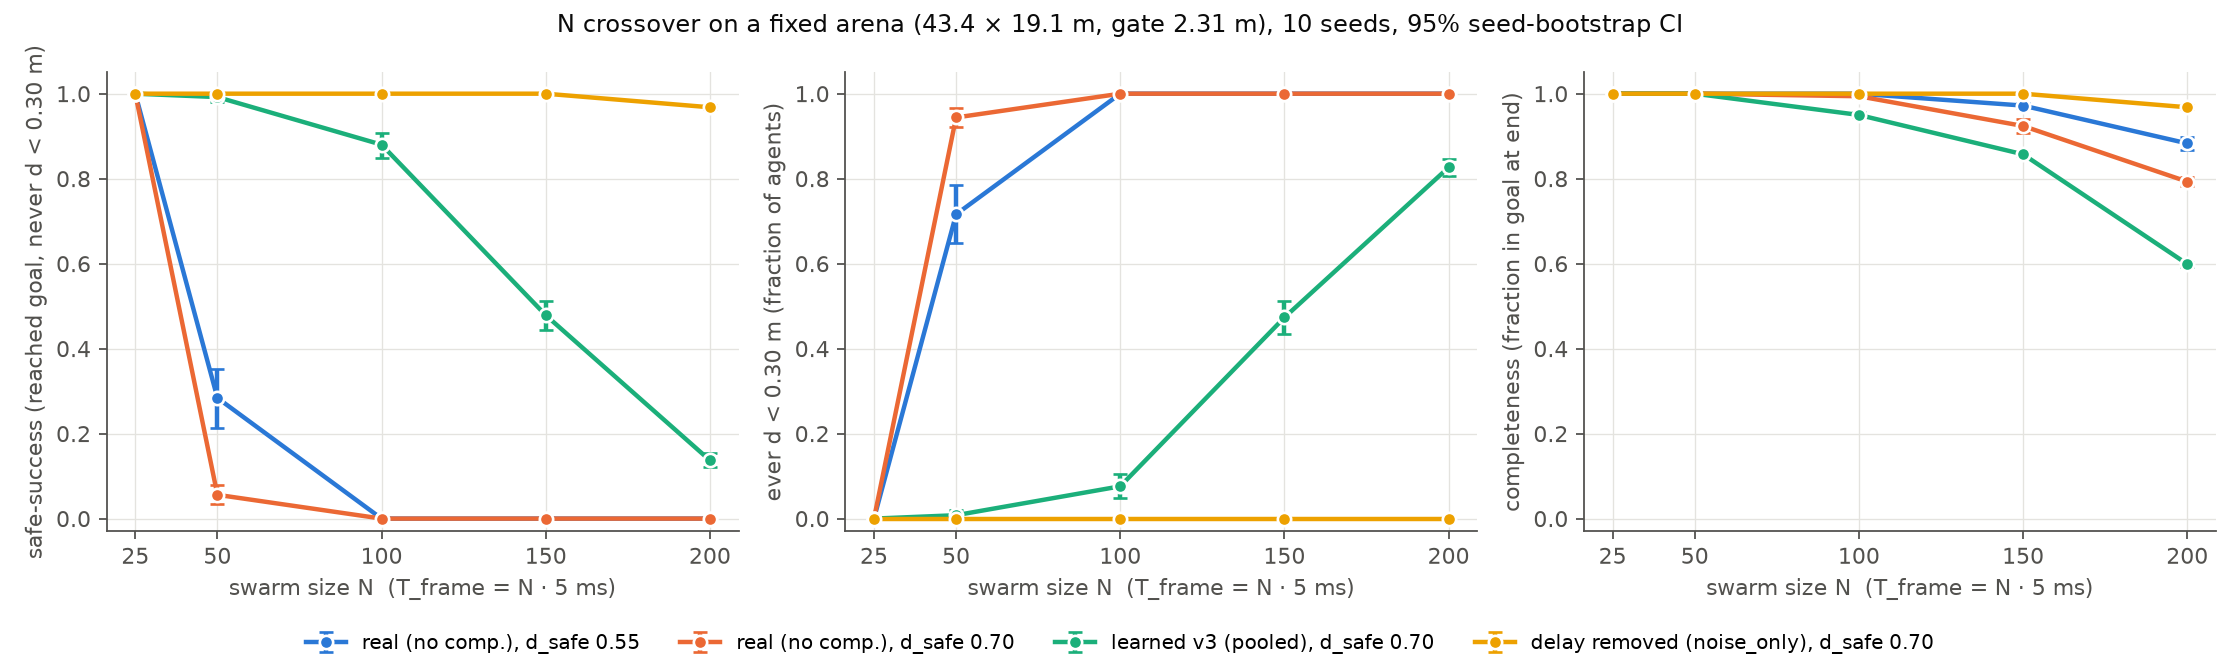
\includegraphics[width=\columnwidth]{fig1_N_crossover.png}
\caption{$N$ crossover (Config G, @T metric; regeneration under the settled metric pending).
Removing the delay (noise\_only) keeps every agent collision-free up to $N=200$.}
\label{fig:crossover}
% SRC: results/overnight_figures/fig1_N_crossover.png (data: figure_data.csv fig1_crossover)
\end{figure}

\paragraph{Pure staleness at fixed $N$.}
To separate staleness from density, we fix $N=100$, the geometry and the start packing, and vary
only $\tslot\in\{2.5,5,7.5,10\}$\,ms, i.e.\ $\Tf\in\{0.25,0.5,0.75,1.0\}$\,s. Learned safe@T falls
from 0.986 to 0.892, 0.545 and 0.178. The stale swarm collides at every $\Tf$ (ever $=1.000$).
Learned minus real is $+0.986$, $+0.892$, $+0.545$, $+0.178$, and every CI excludes 0.
% SRC: logs/overnight/review_amend26.md data (result commit ac32b09); figure_data.csv fig5_tslot
\emph{Decomposition.} At equal $\Tf$, the learned ever-collided at fixed $N=100$
(0.014 / 0.072 / 0.455 / 0.822) equals the value from the $N$-sweep at $N=\Tf/5$\,ms
(0.008 / 0.076 / 0.473 / 0.827) within CI at all four points. This holds although $N$, packing and
neighbour count differ by up to $2\times$. Learned completeness, in contrast, stays at
0.958--1.000 at fixed $N$ but falls to 0.857 / 0.599 at $N=150/200$.
% SRC: logs/overnight/review_amend26.md Q3 table
For the compensated swarm, \emph{collisions track staleness and completeness tracks density}.
For the uncompensated swarm the number of neighbours also matters. At $\Tf=0.25$\,s it collides
everywhere at $N=100$ (ever 1.000), against 0.944 at $N=50$ ($\dsafe=0.70$). The stale swarm is
unsafe either way.
% SRC: review_amend26 Q3 table (real 0.70: 1.000 / 0.944) and Step A last bullet

\paragraph{Gate width is a weak lever.}
At $N=100$ we vary the gate from 1.5 to 7.0\,m, a $4.7\times$ change in gate flux (66.7 to 14.3
agents/m). The stale swarm collides at every gate. Learned ever-collided stays within 0.07--0.13,
and only the 1.5\,m gate is measurably worse (0.126\ci{0.107}{0.147} vs 0.072 at 3.5 and 7.0\,m).
Learned minus real safe@T is $+0.874$ to $+0.928$ at every gate. The open-loop error ratio is flat
at 0.52--0.53, so gate flux does not change the estimation error that drives collisions.
% SRC: logs/overnight/review_amend25.md data + open-loop table (result commit 1ce2b21); figure_data.csv fig4

\subsection{Compensation recovers safety, and only through the CBF}
\label{sec:layers}
\emph{[Links 3--4: compensation restores; each layer earns its place.]}

\paragraph{Compensation in the $N$-sweep (Config G, @T).}
At matched margin (0.70), learned minus real safe@T is $+0.936$\ci{0.912}{0.960} at $N=50$,
$+0.880$\ci{0.848}{0.908} at 100, $+0.479$\ci{0.445}{0.511} at 150 and $+0.137$\ci{0.121}{0.154} at 200.
% SRC: logs/overnight/review_amend22.md Differences (commit c24e62f)
The learned predictor therefore recovers 0.99 / 0.88 / 0.48 / 0.14 of the noise\_only$-$real gap
at $N=50/100/150/200$. Classical compensators fail here. cv amplifies broadcast noise
(safe@T 0.000 at $N=50$, below the uncompensated 0.284). The congestion-blind Smith-type
predictor places phantom neighbours in the gate, and the swarm locks up (completeness 0.00--0.05 at
$N\ge100$). A noise-optimal classical baseline on the same four-broadcast window has been
specified but not run (Sec.~\ref{sec:limits}).
% SRC: logs/overnight/review_amend27.md Q2 + Smith section + "Fairness consequence" (commit 2edfe32)
The headroom left above v3 is $+0.120$\ci{0.092}{0.153}, $+0.521$ and $+0.831$ safe@T at
$N=100/150/200$ (noise\_only minus learned).
% SRC: logs/overnight/review_amend24.md noise_only - learned table

\paragraph{Layer split.}
We feed the compensated (or oracle) estimate to one layer only and the stale estimate to the other.
In Config G at the @T metric (Table~\ref{tab:layers}, top), compensation fed \emph{only} to the MFG
density term changes safe@T by exactly $0.000$\ci{0}{0} relative to no compensation, at every
$N$, for both the learned and the oracle estimate. Fed only to the CBF, it recovers
104\% / 105\% / 72\% (learned) and 100\% / 100\% / 100\% (oracle) of the both-layers gain at
$N=100/150/200$.
% SRC: logs/overnight/review_amend27.md Q3 (commit 2edfe32)
The MFG-only zero is metric-independent: in those cells every agent collides, so the settled
upper bound $1-\text{ever}$ is exactly 0.
% SRC: results/amend38_settled_recompute/report.json A1_bound/amend27/cells/N*/split_learned-real_d0.70 (safe_settled_upper_bound 0.0)
In Config S, where trajectories exist, the split is recomputed exactly under the settled metric
(Table~\ref{tab:layers}, bottom). An oracle-clean CBF with a delayed MFG gives $+0.802$\ci{0.788}{0.818}
safe-settled over the stale swarm, matching full delay removal ($+0.800$). A clean MFG with a
delayed CBF gives $+0.000$\ci{0}{0}. Safety is identical under both metrics in all 51 Config S
rollouts.
% SRC: logs/overnight/review_amend38.md A2 + relative claims; results/amend38_settled_recompute/report.json A2_contrasts (commit c201490)

\begin{table}[t]
\centering\small
\setlength{\tabcolsep}{3.5pt}
\resizebox{\columnwidth}{!}{\begin{tabular}{lcccc}
\toprule
\multicolumn{5}{l}{\emph{Config G, $\dsafe=0.70$, safe@T (10 seeds)}}\\
$N$ & MFG-only & CBF-only & both & none (real)\\
\midrule
100 learned / oracle & 0.000 / 0.000 & 0.918 / 1.000 & 0.880 / 1.000 & 0.000\\
150 learned / oracle & 0.000 / 0.000 & 0.503 / 1.000 & 0.479 / 1.000 & 0.000\\
200 learned / oracle & 0.000 / 0.000 & 0.098 / 0.965 & 0.137 / 0.968 & 0.000\\
\midrule
\multicolumn{5}{l}{\emph{Config S, $N=100$, $\dsafe=0.55$, oracle (noise\_only), safe settled 5\,s (5 seeds)}}\\
& 0.000 & 0.802 & 0.800 & 0.000\\
\bottomrule
\end{tabular}}
\caption{Layer split. ``MFG-only'' feeds the compensated (or oracle) estimate to the MFG density term
and the stale estimate to the CBF; ``CBF-only'' does the reverse.}
\label{tab:layers}
% SRC: review_amend27.md Q3 (Config G); review_amend38.md A2 table (Config S: split rows, noise_only, real)
\end{table}

At $N=100$ in Config G, the CBF-only learned split is \emph{above} feeding both layers by
$+0.038$\ci{0.006}{0.074}. At $N=200$ it is below, by $-0.039$\ci{-0.059}{-0.020}. The MFG-layer
share is small in both directions.
% SRC: review_amend27.md Q3 bullets
An exploratory CPU run in Config S (5 seeds) gives the same picture for collisions and arrival
together. Removing the delay from the CBF inputs alone recovers 100\% of the collision measures and
96\% of reached-goal. Removing it from the MFG density term alone reduces collision pair-steps by
15\% (5/5 seeds) but prevents not a single agent from colliding.
% SRC: logs/overnight/review_amend34.md "Recovered fraction" + Readings (commit d28afa2)

\paragraph{What the MFG layer is for.}
The MFG layer earns its place through liveness. In Config S with exact positions, the full MFG+CBF
controller settles 0.920 of the swarm, against 0.602 for a CBF-only controller that uses decoupled
single-agent routing. The difference is $+0.318$\ci{0.274}{0.370}, and both arms have zero
collisions. CBF-only agents are frozen outside the goal rather than moving in and out: their
success is identical at every window length.
% SRC: review_amend38.md A2 (fresh 0.920, fresh_nomfg 0.602) + report.json A2_contrasts "fresh - fresh_nomfg"; review_amend37 (CBF-only window-invariant)
Conversely, the MFG without the CBF reaches the goal (completeness 1.000) but 99.8\% of agents
collide, so the CBF is necessary for safety.
% SRC: review_amend38.md A2 (fresh_nocbf 1.000 / 0.002 / ever 0.998)

\paragraph{Learned compensation under the settled metric (Config S).}
In Config S, learned minus real is $+0.154$\ci{0.106}{0.208} safe-settled ($+0.168$ @T). The
relative claim holds, but the absolute recovery is much smaller than in Config G: 0.154 of a
0.800 gap.
% SRC: report.json A2_contrasts "learned - real" safe_settled_5s; review_amend38 A2
The Config S learned predictor is the earlier $N=100$-only model of that configuration, not v3.
% SRC: prereg/prereg_projectA_amend34_layer_delay_cpu.md L37 (2x64 MLP, train_predictor.py); review_amend34 link 3
In the delayed arms, settled completeness is about 0.29 below completeness@T (real 0.718 $\to$
0.426), because those agents churn in and out of the disc. Completeness@T overstates arrival for
every delayed arm.
% SRC: review_amend38.md "How much absolute completeness drops"

%=====================================================================
\section{Evaluation Metric: Settled Arrival and the Rim}
\label{sec:metric}
%=====================================================================
\emph{[Link 1: delay-free works --- not met in full.]}

Scoring arrival at a single instant $T$ rewards transients. In Config S, adding a terminal goal
cost to the MFG raised completeness@T of the oracle swarm from 0.934 to 0.994. Fourteen to eighteen
agents were still outside the disc 1\,s before $T$ and rushed in during the last half second.
% SRC: review_amend36.md (commit 50cbf6e) flag table
Under the settled metric that controller was \emph{worse} by about 0.10 (fresh $-0.106$\ci{-0.116}{-0.096}),
and it was reverted by a pre-registered rule.
% SRC: review_amend37.md (commit 814bd2d)
We adopt the settled metric (inside in at least 90\% of the last 5\,s) as the standard.
Verdicts are identical at 3\,s and 10\,s.

\paragraph{Delay-free success is limited by the goal rim.}
Even without delay, the swarm does not fully settle. Safe settled is 0.920 with exact positions and
0.800 with sensor noise, with zero collisions in both cases.
% SRC: review_amend37.md / review_amend38.md A2
The non-settlers are not stuck far away. All 40 exact-position non-settlers (8 per run) end within
0.30\,m of the 4.20\,m rim, at a median of 0.18\,m outside. Half of them oscillate across the rim.
30\% are parked because the MFG gives almost no inward push there (median radial command
$-0.02$\,m/s): at the rim, goal attraction and crowd aversion balance. Only 3 of the 40 are
blocked by the CBF. With sensor noise, the outer ring jitters instead: 59\% of non-settlers
oscillate, crossing the rim a median of 7 times in 5\,s, as the CBF cuts an inward MFG command of
$-0.40$ to $-0.13$\,m/s. At most 12\% of non-settlers are still approaching, and those are already
inside at $T$, so a longer horizon is not expected to help.
% SRC: review_amend38.md B table + "Where they are" + "Mechanism" (commit c201490); report.json B (d_T quantiles)
The shortfall is a property of the equilibrium formation, whose outer ring lies on the disc
boundary. It is not a delay effect.

\paragraph{A goal-tolerance band (to be computed).}
The non-settlers sit about one drone body (0.30\,m) outside the disc. We therefore propose to
report safe-settled success also with a goal tolerance of $D_{\mathrm{COLL}} = 0.30$\,m added to the
radius. This band has \textbf{not yet been computed}; it will be evaluated from the existing
Config S logs and in the regenerated Config G cells. One consequence is already fixed by a bound
that holds for any tolerance. Safe success of an agent requires that it never collided, so
$\text{safe} \le 1 - \text{ever}$. In Config S that caps the stale swarm at $0$
(ever $=1.000$) and the learned swarm at $1-0.734 = 0.266$, while the delay-free arms are uncapped
(ever $=0$). However generous the arrival criterion, it cannot remove the damage the delay does to
safety.
% SRC: review_amend38.md A1 bound logic + A2 ever_collided column (real 1.000, learned 0.734, noise_only/fresh 0)

%=====================================================================
\section{Negative Result: A Conformal $\sigma$-CBF Does Not Beat a Constant Margin}
\label{sec:sigma}
%=====================================================================
\emph{[Link 4 for a predictor-driven margin layer: not earned.]}

\paragraph{Idea.} Replace the constant margin with a per-neighbour one,
$\dsafe^{ij} = \max\big(\text{floor},\,D_{\mathrm{COLL}} + k\,q_\alpha\,\sigma_{ij}\big)$. Here $\sigma_{ij}$ is
a learned estimate of v3's position error for neighbour $j$, and $q_\alpha$ is a conformal
quantile. Each stage was gated by a criterion fixed before its data existed.
% SRC: control/cbf.py L56 (sigma mode); logs/overnight/phaseB_gpred_gate.md (commit b020562)

\paragraph{G-pred: the error model ranks risk but does not size it.}
On held-out closed-loop learned trajectories (pairs closer than 2\,m), the error model identifies
the top-10\% errors with AUC 0.781--0.863 across $N$ (pooled 0.907). At $N\ge100$, 77--84\% of the
top-1\% errors fall in the top-1\% of predicted $\sigma$. The registered gate passed. Error
\emph{magnitude}, however, is poorly explained: pooled $R^2_{\log} = 0.346$ and per-$N$
0.146--0.280. Within the top decile, $R^2_{\log}$ is negative at every $N$. The model knows
\emph{which} neighbours are risky, not \emph{how} far off the worst ones are.
% SRC: logs/overnight/review_gpred.md PRIMARY table + Tail (result commit 01701ef)

\paragraph{G-cal: calibration holds offline.}
With (N, $\sigma$-quintile) binned split-conformal calibration, marginal coverage is within
tolerance at every $N$ and $\alpha$. The worst conditional decile at $\alpha=0.10$ is 0.876.
Offline coverage at $\alpha=0.05$ is 0.955. Plain per-$N$ calibration under-covered low-$\sigma$
pairs at $N=200$ (0.842); that was fixed by the registered binning.
% SRC: logs/overnight/review_amend31.md G-cal table + "Where the guarantee's premise holds/breaks"

\paragraph{G-win: no gain over the constant-margin frontier.}
The registered test compares the primary arm ($\alpha=0.05$, binned) against the \emph{best}
constant margin per $N$ and requires a positive lower CI at both $N=150$ and 200. The first run
failed ($-0.159$ and $-0.188$). It also had an unbounded margin (realized mean $\dsafe$ up to
$2.8\cdot10^5$\,m in one step at $N=200$).
% SRC: review_amend31.md G-win (report commit 29e1496) + Classification
We re-ran it once with the margin capped at 1.5\,m. That was the only code change, verified
bit-equal with the cap disabled. The capped $\sigma$-CBF gives $+0.039$\ci{+0.005}{+0.075} safe@T
over the best constant margin (0.85) at $N=150$, with $+0.281$ completeness. At $N=200$ it gives
$-0.189$\ci{-0.200}{-0.177} against the best constant margin (1.00), with every agent colliding
in every $\sigma$ arm. \textbf{Verdict: not met.}
% SRC: logs/overnight/review_amend35.md G-win table + S2 sanity (report commit 14049bb); results/amend35_sigma_cap/report.json
The capped run used a different GPU (RTX PRO 6000) from the A100 runs, and all constant-margin
comparators were re-run on that GPU.
% SRC: review_amend35.md Infra

\paragraph{The guarantee does not survive closed loop.}
At $N=200$ the closed-loop coverage of the $\sigma$ margin is 0.77 on pairs closer than 2\,m and
0.69 on rows where it binds, against 0.95 offline. At $N=150$ it is 0.94 and 0.89.
% SRC: review_amend35.md "Closed-loop coverage"; report.json rows/*/sigma_bin_a0.05/sigma_cov_rows_near2m, sigma_cov_binding
The margin changes the swarm's behaviour, so the controller's own trajectories are no longer
exchangeable with the calibration data.

\paragraph{Why it helps at $N=150$ and fails at $N=200$ (interpretation).}
At $N=150$ the margin is selective. It binds on 12.6\% of CBF rows, with mean $\sigma$ 0.30\,m and
mean $\dsafe$ 0.725\,m. Extra clearance goes to a few risky neighbours, which is the only regime in
which a ranking-only error model can pay off. At $N=200$ it binds on 75.2\% of rows, with mean
$\sigma$ 0.64\,m and mean $\dsafe$ 0.959\,m. It then behaves like a broad, large constant margin
applied to estimates that are now out of calibration. That is the regime in which a larger margin
on a poor estimate hurts (Sec.~\ref{sec:method}).
% SRC: results/amend35_sigma_cap/report.json rows/{150,200}/sigma_bin_a0.05 (sigma_bind_frac 0.126/0.752, sigma_mean_rows_m 0.304/0.638, d_safe_mean 0.725/0.959)
This concentrated-versus-broad reading fits the numbers, but it is an interpretation and has not
been tested by a dedicated experiment.

%=====================================================================
\section{Limitations}
\label{sec:limits}
%=====================================================================
\begin{itemize}
\item \textbf{No hard guarantee.} The CBF certifies separation with respect to \emph{estimated}
  positions. Under delay no margin we tested is both collision-free and complete at $N\ge100$ with
  the learned predictor. The only way below ever 0.02 at $N=100$ was to freeze the swarm
  (completeness 0.764).
  % SRC: review_amend23 Step C/E
\item \textbf{Single geometry.} One single-gate scenario (two parameterizations) with 5-inch drone
  parameters. Multi-gate, corridor and obstacle-rich scenarios from the original design were not run.
  % SRC: prereg/prereg_projectA.md Sec.5 (4 scenarios planned); CLAUDE.md (single-gate kept)
\item \textbf{Completeness ceiling at the rim.} Delay-free settled success is 0.920 (exact) and
  0.800 (noisy) (Sec.~\ref{sec:metric}). The PI's success criterion (every drone arrives) is not met
  by any arm, including the oracle.
\item \textbf{Lost raw data; metric regeneration.} Trajectories of the Config G crossover, mechanism
  control and $\tslot$ sweep were deleted with the compute volumes. Their safety numbers
  (ever-collided) are metric-independent. Their success and completeness numbers are @T and are
  being regenerated under the settled metric. Only Config S ($N=100$) is verified under the settled metric.
  % SRC: review_amend38.md "Data limit"
\item \textbf{Classical baseline.} cv and Smith fail for identifiable reasons (noise
  amplification; congestion-blind model). A noise-optimal least-squares constant-velocity fit on the
  NN's own four-broadcast window has been specified but not run. ``NN beats classical
  compensation'' is therefore stated only against these two comparators.
  % SRC: review_amend27 "Fairness consequence"; prereg/prereg_projectA_amend32_cvls.md (registered, not run)
\item \textbf{Statistics and determinism.} Config S has 5 seeds, so a paired sign-flip test cannot
  reach $p<0.05$ ($p_{\min}=0.0625$). The learned GPU path is not bit-deterministic across runs:
  the $N=100$ cell replicated as 0.892 vs 0.880, within CI.
  % SRC: review_amend34 Statistics; review_amend23 Step B.1
\item \textbf{Offline MFG.} The equilibrium is solved offline per $N$ (stage 1). The online
  per-drone MFG with dynamic waypoints and unknown terrain is not addressed.
\end{itemize}

%=====================================================================
\section{Conclusion and Next Steps}
%=====================================================================
In a two-layer MFG+CBF swarm with drone-sized keep-out distances, UWB/vision noise and TDMA delay,
collisions are caused by stale neighbour estimates, not by density. Removing the delay removes
every collision up to $N=200$, and a pure-staleness sweep reproduces the collision rate of the
$N$-sweep. Compensation belongs in the CBF layer. Fed to the MFG density term it is worth exactly
zero, even as an oracle. The MFG layer earns its place through liveness instead. A conformally
calibrated, learned uncertainty margin does not move the constant-margin frontier, and its
coverage breaks in closed loop.

Two directions follow; neither is a result of this paper.
(a) \emph{Harder geometries.} With one gate, routing is nearly trivial. The MFG's advantage in
throughput and liveness should matter more where routing is non-trivial (several gates,
obstacles), and that is where an MFG-layer use of compensation could still be tested.
(b) \emph{Recovering safety at large staleness.} At $\Tf \ge 0.75$\,s even the learned
compensator leaves most of the gap (0.48 and 0.14 recovered at $N=150/200$). Candidate fixes act on
the cause rather than the margin. Staleness-aware routing would keep agents with old information
apart. Event-triggered or priority TDMA slots would shorten the age of the neighbours that are
closing.
Before either, the Config G cells will be regenerated under the settled metric and the goal-tolerance
band, and the noise-optimal classical baseline will be run.

\bibliographystyle{named}
\bibliography{refs}

\end{document}
